\documentclass[a4paper,12pt]{article}

\usepackage{graphicx}
\title{FAN simulator manual}
\author{D. Najder, J. Palider}
\date{Krak\'ow, \today}

\begin{document}

	\maketitle

	\newpage
	
	\section{Running \emph{FAN simulator} v.1.0}
	
	The very first step to use \emph{FAN simulator} is to get it. The most common
	way to do that is to download either the source code from the project site
	under svn control at \emph{https://fansimulator.googlecode.com/svn/trunk} or the
	.jar packages that contain all necessary libraries to run the application
	successfully under both Windows or Linux. Each package is prepared for one of
	the operating systems.	
	
	\emph{FAN simulator} has been written with portability in mind. That is why
	Java has been chosen as the programming language. Despite that, there are
	certain requirements that must be met. First of all, JVM~6.0 must be available, Java
	native algorithms in versions 5.0 and 6.0 generate different internal states
	which in some configurations results in crashing the application.

	For executable packages, nothing but JVM is needed. However, the following
	packages must be available to build and run the application from sources
	\emph{(some older versions should also work, but were not tested)}:
	\begin{enumerate}
	\item {SWTv3.3.2 for the target platform}
	\item {jcommon v1.0.10}
	\item {jfreechart v1.0.6}
	\end{enumerate}
	
	
	\section{User manual}
	This section will describe all the functionality that GUI of \emph{FAN
	simulator} provides. It will show how to deal with the application and guide
	through all the windows and sub-windows that might be displayed to the user
	while working with \emph{FAN simulator}.
	Blue rectangles on screenshots with corresponding numbers were postprocessed
	to easier identify graphical objects. They will be called \emph{regions}.

	A group of simulation parameters that control simulation behaviour will be
	called the simulation scenario, or simply scenario. There are two ways of
	setting simulation scenario. One is by creating an \emph{.xml} file containing
	necessary information enclosed by XML tags and then loading it or by creating
	the scenario from within the \emph{FAN simulator} application. 
	The primary task while constructing a simulating scenario is to define at
	least two servers (one server works but gives no results) which are
	going to participate in packet transmission, set a link between them (actually
	a one-way interface to the destination server), configure FAN router
	parameters and creating a traffic generator adjacent to a server.
	
   \subsection{Creating scenario file manually}
	\label{MANUALCREATION}
    Here is a skeleton of a minimal scenario file. The listing below can be
    easily generated from GUI, at this point, however, its structure is
    described.
    \begin{verbatim}

 1.   <?xml version="1.0" encoding="UTF-8"?>
 2.   <root>
 3.      <description>
 4.          This is a sample description for non-existing scenario.
 5.          It can span over several lines and theoretically be as
 6.          long as necessary!
 7.      </description>
 8.      <server n="Server nr 1">
 9.          <interface	 bandwidth="320000"
10.                      maxFlowListSize="25"
11.                      maxPL="0.1"
12.                      minFR="16000"
13.                      peer="Server nr 2"
14.                      probability="1.0"
15.                      queueSize="80000"
16.          />
17.          <generator  type="constant">
18.              <packetSize>400</packetSize>
19.              <startTime>0.0</startTime>
20.              <flowLowerRange>1</flowLowerRange>
21.              <flowHigherRange>20</flowHigherRange>
22.              <looped>true</looped>
23.              <interval>0.00125</interval>
24.          </generator>
25.      </server>
26.      <server n="Server nr 2">
27.          <interface  bandwidth="1" 
28.                      maxFlowListSize="100"
29.                      maxPL="1.0"
30.                      minFR="1.0"
31.                      peer="Server nr 2"
32.                      probability="1.0"
33.                      queueSize="100000"
34.          />
35.      </server>
36.  </root> 

	\end{verbatim}
 
	Each scenario file should be a properly formatted \emph{.xml} file. Line 1
	consists of a comment including coding type used in that document.\\
	Lines 2 and 36 are the root tags, by convention named \emph{root}. It is
	obligatory to have them in the scenario file.\\
	Lines 3 and 7 denoted as \emph{description} tag enclose some
	additional text, usually a description of a scenario. As this is an XML file,
	some characters are forbidden -- XML documentation gives further
	information about that issue.\\
	\emph{Server} tag embracing lines 8-25 sets a server name and describes its
	behaviour. Child nodes that might appear in the \emph{server} section can be
	\emph{interface} or \emph{generator}.\\
	The \emph{interface} tag does not have any sub-tags, as all the necessary
	information is represented as attributes of the tag. These are:
	\begin{enumerate}
      \item bandwidth -- bandwidth in B/s of a link from \emph{this} interface
      to the destination server
      \item maxFlowListSize -- the total number of flows kept in FAN router
      \item maxPL -- maximum priority load of a flow
      \item minFR -- minimum fair rate of a flow
      \item peer -- name of a server this interface in liked to
      \item probability -- probability that a packet while being
      statistically routed (no real routing algorithms are implemented) will
      be switched to this interface. A sum of \emph{probability} over all
      \emph{interfaces} on a server must be equal to 1.0.
      \item queueSize -- maximum size in B of a queue that keeps packets
      waiting for transmission
    \end{enumerate}
    \emph{Generator} tag describes traffic sources. There are four types of
    traffic generators (time values are given in seconds):
    \begin{enumerate}
      \item constant -- packets are sent every \emph{interval} 
      \item uniform -- packets are sent in various intervals between
      \emph{StartRange} and \emph{EndRange}
      \item normal -- packets are sent in time spaces accordingly to Gaussian
      distribution configured with \emph{mean} and \emph{variance}. 
      \item basic -- TODO
    \end{enumerate}
    
    Apart from specific parameters of generators' types, there are a few
    additional ones:
    
    \begin{enumerate}
      \item packetSize -- defines a size of every generated packet, does not
      change for particular simulation
      \item startTime -- specifies where a generator starts creating packets
      \item stopTime (optional) -- if a generator is to stop at a particular
      point in time, this field should be set. By default packets are generated
      from \emph{startTime} till the simulation end.
      \item flowLowerRange -- with \emph{flowHigherRange (see below)} defines a
      range of flow identifiers that are randomly generated. If there is a need
      to generate packets with exactly one flow identifier,
      \emph{flowLowerRange} should be equal to \emph{flowHigherRange}
      \item flowHigherRange -- see \emph{flowLowerRange}
      \item looped -- must be true if \emph{stopTime} is not set 
    \end{enumerate}
    Notice: locally serviced packets are immediately removed from server, thus
    if for a local interface (looping to the server an interface is assigned to)
    \emph{probability} in line 32 is set to 1.0 \emph{bandwidth} may be set to
    any integer value, here 1 as in line 27.
    
	\subsection{Creating scenario from GUI}
	Usually, the easiest way of creating a scenario is to use GUI. Having the
	knowledge of how a scenario is built and what certain scenario parts do, it
	is just a matter of filling empty gaps.
	
	\subsubsection{Main window}
		Creating scenario from \ref{MANUALCREATION} in GUI will be presented here.
		
		\begin{figure}[h]
		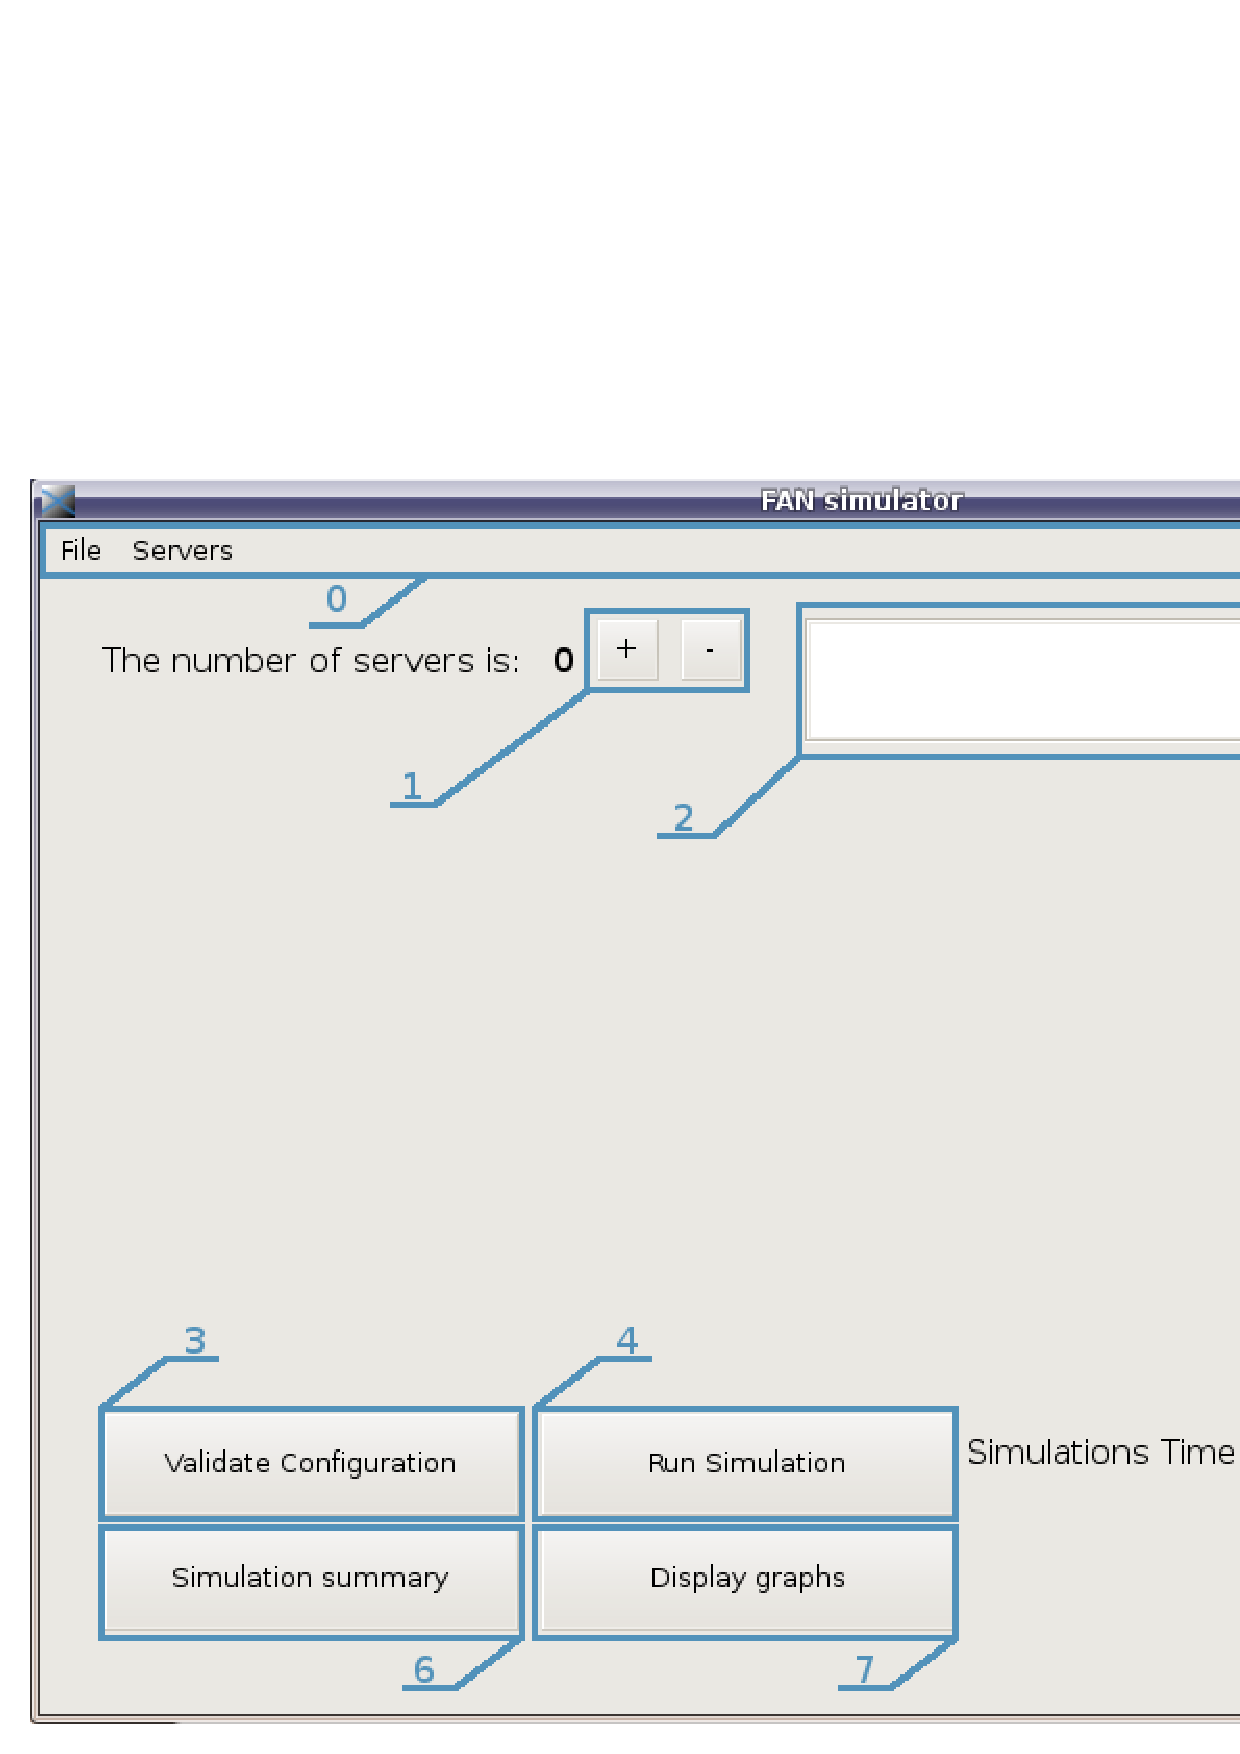
\includegraphics[width=150mm]{man/MainWindow.png}
		\caption{Main FAN simulator window}
		\label{MAINWINDOW}
		\end{figure}
	
		Figure \ref{MAINWINDOW} presents the main window of an application that is
		displayed to the user after start\footnote{Just after splash screen disappears}. It
		consist of a menu bar at the top of the window (0) and the main 
		simulation window. The following objects (group of objects) are visible on the
		main simulation window described with the corresponding numbers and their
		functionality:
		\begin{enumerate}
		\item {adds/removes one simulating server}
		\item {text area -- it is a good idea to comment a scenario}
		\item {performs a basic test of simulation configuration; checks if all
		necessary parameters are present}
		\item {starts the simulation}
		\item {defines simulation duration -- represents simulation time in seconds,
		e.g. if there are 10 packets waiting for trasmission and each needs
		100~milliseconds and simulation assumes 1 second duration, 10~packets are
		supposed to be transmited }
		\item {pop-ups a subwindow with simulation results}
		\item {pop-ups a subwindow with simulation graphs -- generates a plot
		of simulation results}
	    \end{enumerate}
    
    \subsubsection{Server tab}
	    
	    As already mentioned in \ref{MANUALCREATION} there should be at least two
	    servers. To achieve this their number should be adjusted by clicking either
	    ''+'' or ''--'' button of region 1 from picture \ref{MAINWINDOW}.
	 	\begin{figure}[cht]
		\includegraphics[width=150mm]{man/ServerTab.png}
		\caption{Main FAN simulator window with server tabs}
		\label{SERVERTAB}
		\end{figure}
	
		Figure \ref{SERVERTAB} presents the main window of an application with example
		tabs that present information of configuration of corresponding servers.
		Visible objects have following functionality:	
		  
		\begin{enumerate}
		\item {opens an interface configuration window}
		\item {removes selected interface from current server}
		\item {opens an generator configuration window}
		\item {removes selected generator from current server}
		\item {display current server configuration}
		\end{enumerate} 

	\subsubsection{Interface configuration window}
	
	Configuration options for an interface are presented in Figure \ref{INTERFACE}.
	These are:
		
		\begin{enumerate}
		\item {value in this field sets interface bandwidth}
		\item {value in this field is needed to routing mechanism }
		\item {value in this field defines queue size}
		\item {value in this field defines Protected Flow List size }
		\item {value in this field specifies the minimum fair rate }
		\item {value in this field specifies the maximum priority load }
		\item {the button applies all the input and selection from this window and
		adds a configured interface to the router}
		\item {selection field which is used to select router to which a connection
		is to be established}
        \end{enumerate} 
        
    and correspond to xml tags introduced in \ref{MANUALCREATION}.
	
		\begin{figure}[cht]
			\begin{center}
			\includegraphics[width=40mm]{man/Interface.png}
			\caption{Interface configuration windows}
			\label{INTERFACE}
			\end{center}
		\end{figure}
	
	\subsubsection{Generator configuration window}
	
	Configuration options for a generator are presented in Figure \ref{INTERFACE}.
	These are:
	
		\begin{enumerate}
		\item {generator type selection:}
			\begin{itemize}
              \item {basic}
              \item {normal}
              \item {constant}
              \item {uniform}
            \end{itemize}
		\item {value in this field declares packet size in bytes }
		\item {value in this field defines when, according to simulation time, the
		generator should start}
		\item {value in this field defines the lower ID for a generated packet }
		\item {if set, tells the gererator when, according to simulation time, to
		stop generating packets }
		\item {value in this field defines the upper ID for a generated packet }
		\item {accepts provided data and creates a generator}
        \end{enumerate} 
        
    and correspond to xml tags introduced in \ref{MANUALCREATION}.
		\begin{figure}[ht]
			\begin{center}
			\includegraphics[width=40mm]{man/Generator.png}
			\caption{Generator configuration windows}
			\label{GENERATOR}
			\end{center}
		\end{figure}

	\subsubsection{Menu bar}
	
	[TODO:]
	Description of menu bar buttons\ldots
	Describing how the simulator works, scenarios,	saving data etc\ldots




	\newpage


\end{document}
